\section{Semantic Multi-Modal Frame Representation}
\subsection{Learning Atoms to Represent Multi-Modal Data}
We represent each frame in our video set as a distribution over set of language and visual atoms. Language atoms are the salient words detected by using a tf-idf like measure, and the visual atoms are found via clustering over object proposals which we extract from frames. We explain the details of finding the atoms and representing the frames in the subsequent sections.
\subsubsection{Learning Language Atoms}
In order to detect salient words, we use tf-idf like measure. For each recipe, we concatanate all subtitles into a single term corpus. As a document corpus, we use all the words extracted from all recipes. Moreover, we compute the tf-idf as $tfidf(w,d,D)=f_{w,d} \times \log \frac{N}{n_{w}}$ where $w$ is the word, $d$ is the corpus of the recipe and $f_{w,d}$ is the frequency of the word in the recipe. Moreover, $N$ represents the total number of videos in all recipes and $n_{w}$ is the number of videos whose subtitle include the word $w$. After computing the tf-idf, we sort all words with their tf-idf values and choose top $K$ words as set of salient words.
\subsubsection{Learning Visual Atoms}
In order to learn visual atoms, we initially generate object proposals from each frame of each videos.
\paragraph{Generating Framewise Object Proposals}
\paragraph{Joint Proposal Clustering to Detect Visual Objects}
\begin{figure}[ht]
  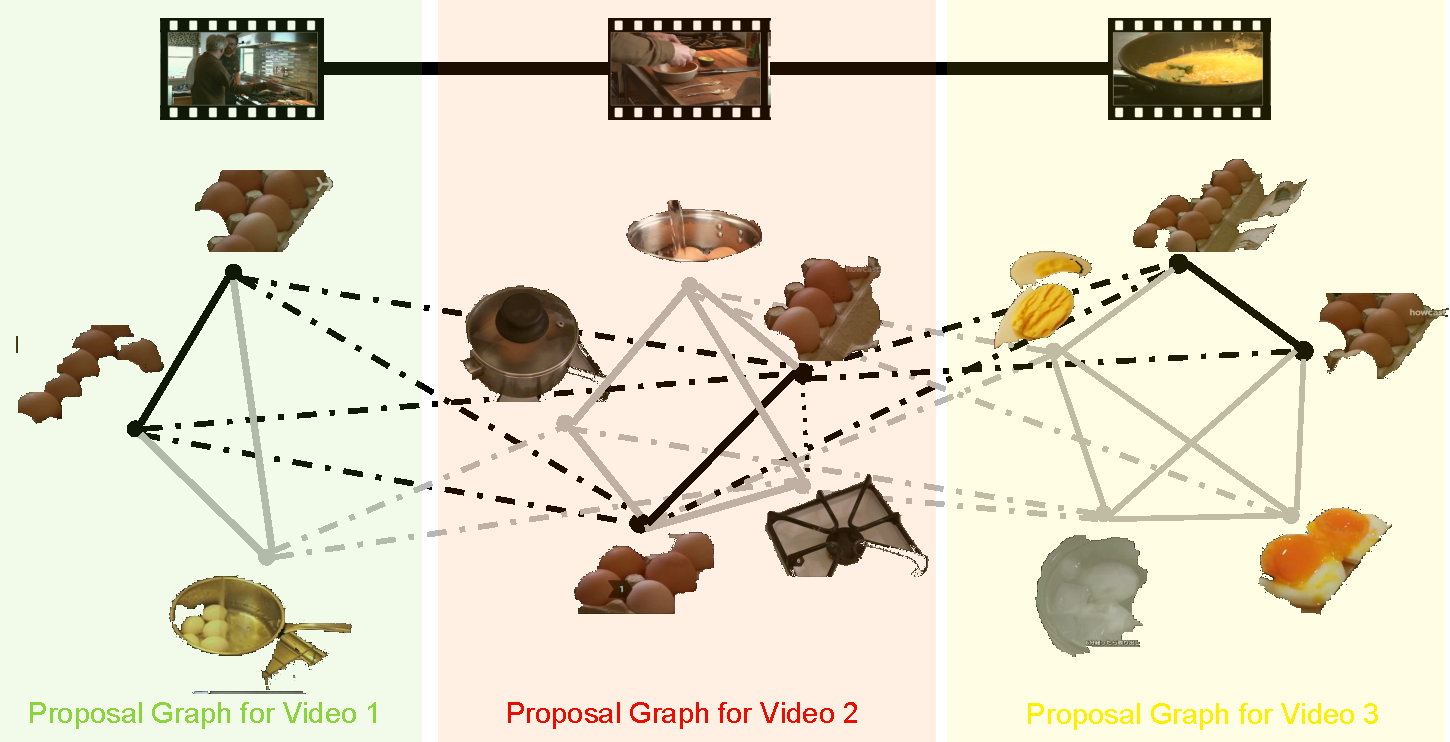
\includegraphics[width=0.48\textwidth]{joint_clustering}
  \scalebox{0.85}{$\arg\max  \color[HTML]{BF9000}{\frac{x_1^TA^(1)x^1}{x_1^Tx^1}}+\color[HTML]{990000}{\frac{x_2^TA^(2)x^2}{x_2^Tx^2}}+\color[HTML]{38761d}{\frac{x_3^TA^(3)x^3}{x_3^Tx^3}}+\color[HTML]{a64d79}{\frac{x_1^TA^(1,2)x^2}{x_1^T\mathds{1}\mathds{1}^Tx^2}}+\color[HTML]{F1C232}{\frac{x_2^TA^(2,3)x^3}{x_2^T\mathds{1}\mathds{1}^Tx^3}}$}
  \caption{Visualization of the joint proposal clustering.}
\end{figure}
\begin{figure}[ht]
  \begin{subfigure}[b]{0.23\textwidth}
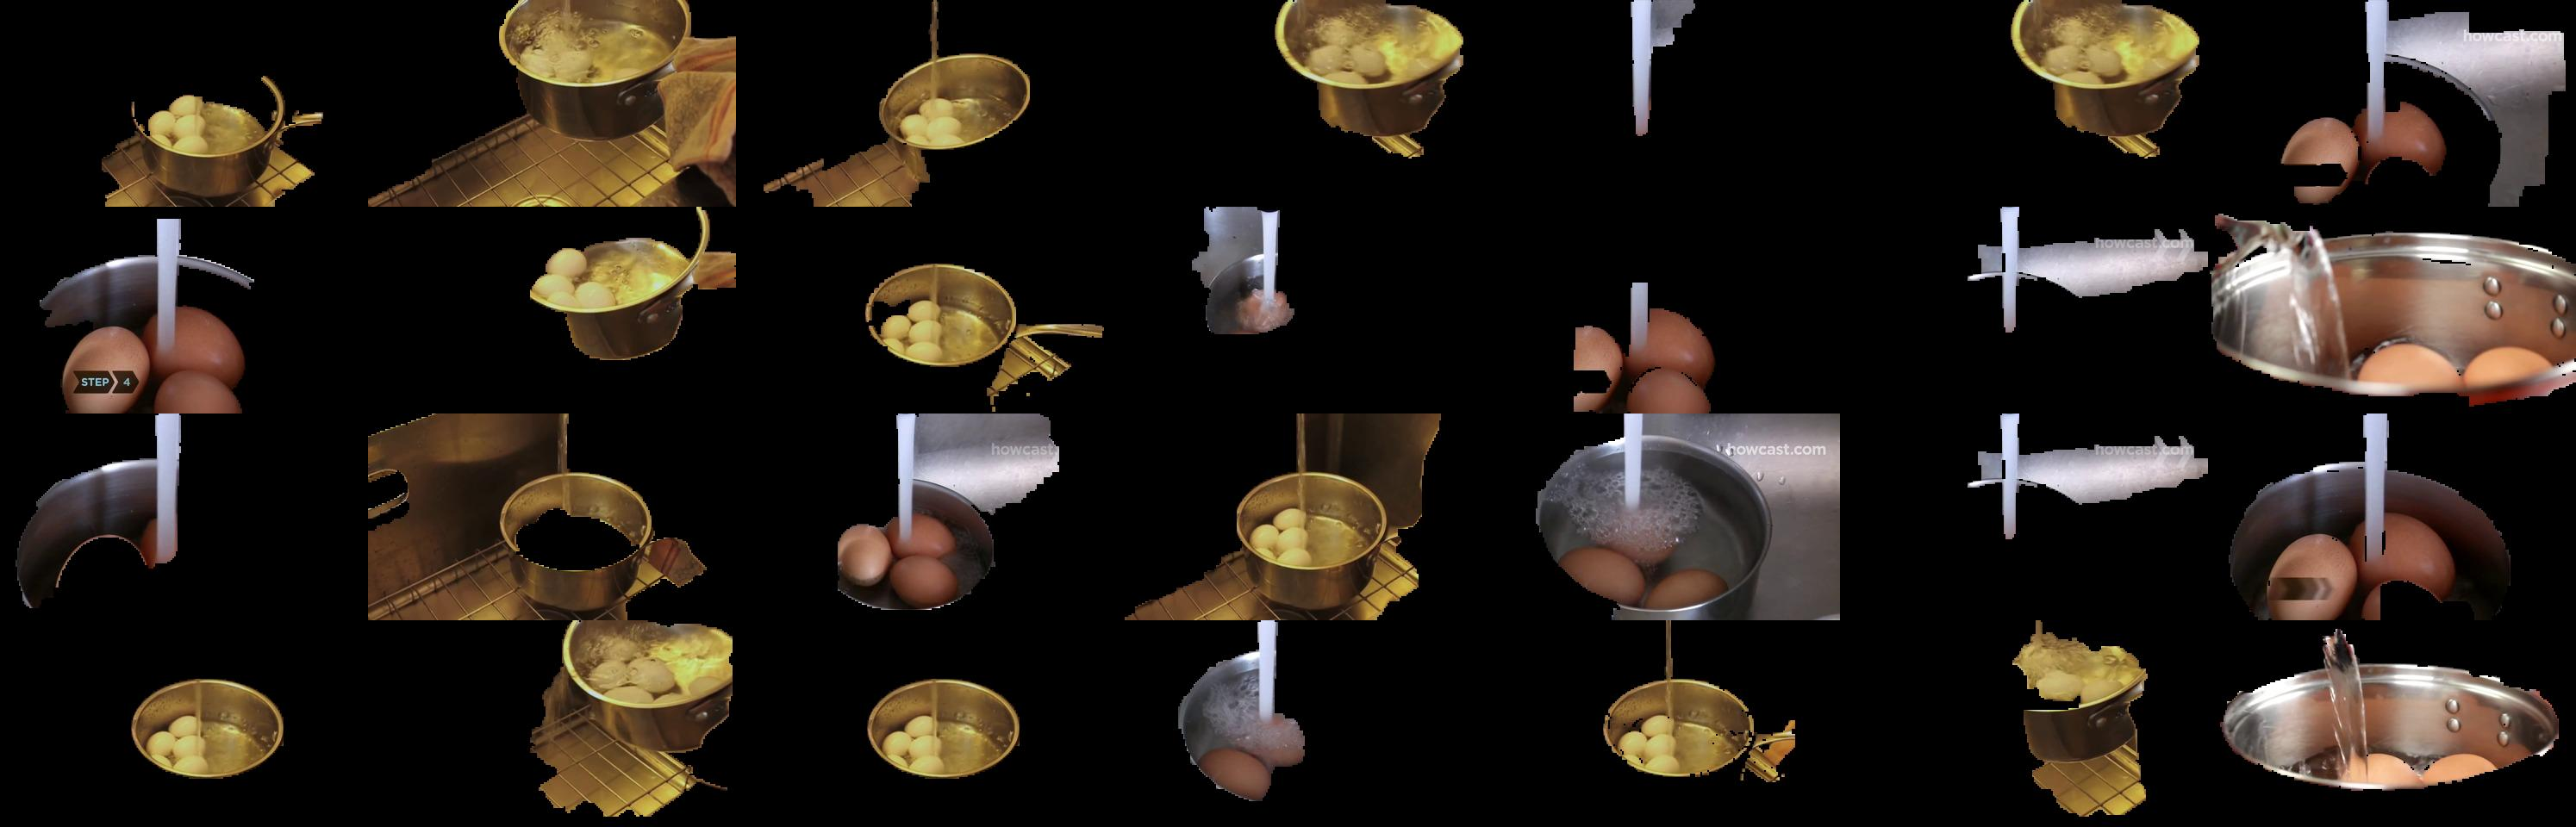
\includegraphics[width=\textwidth]{im0.png}
%\caption{Cluster 1}
\end{subfigure}
~
\begin{subfigure}[b]{0.23\textwidth}
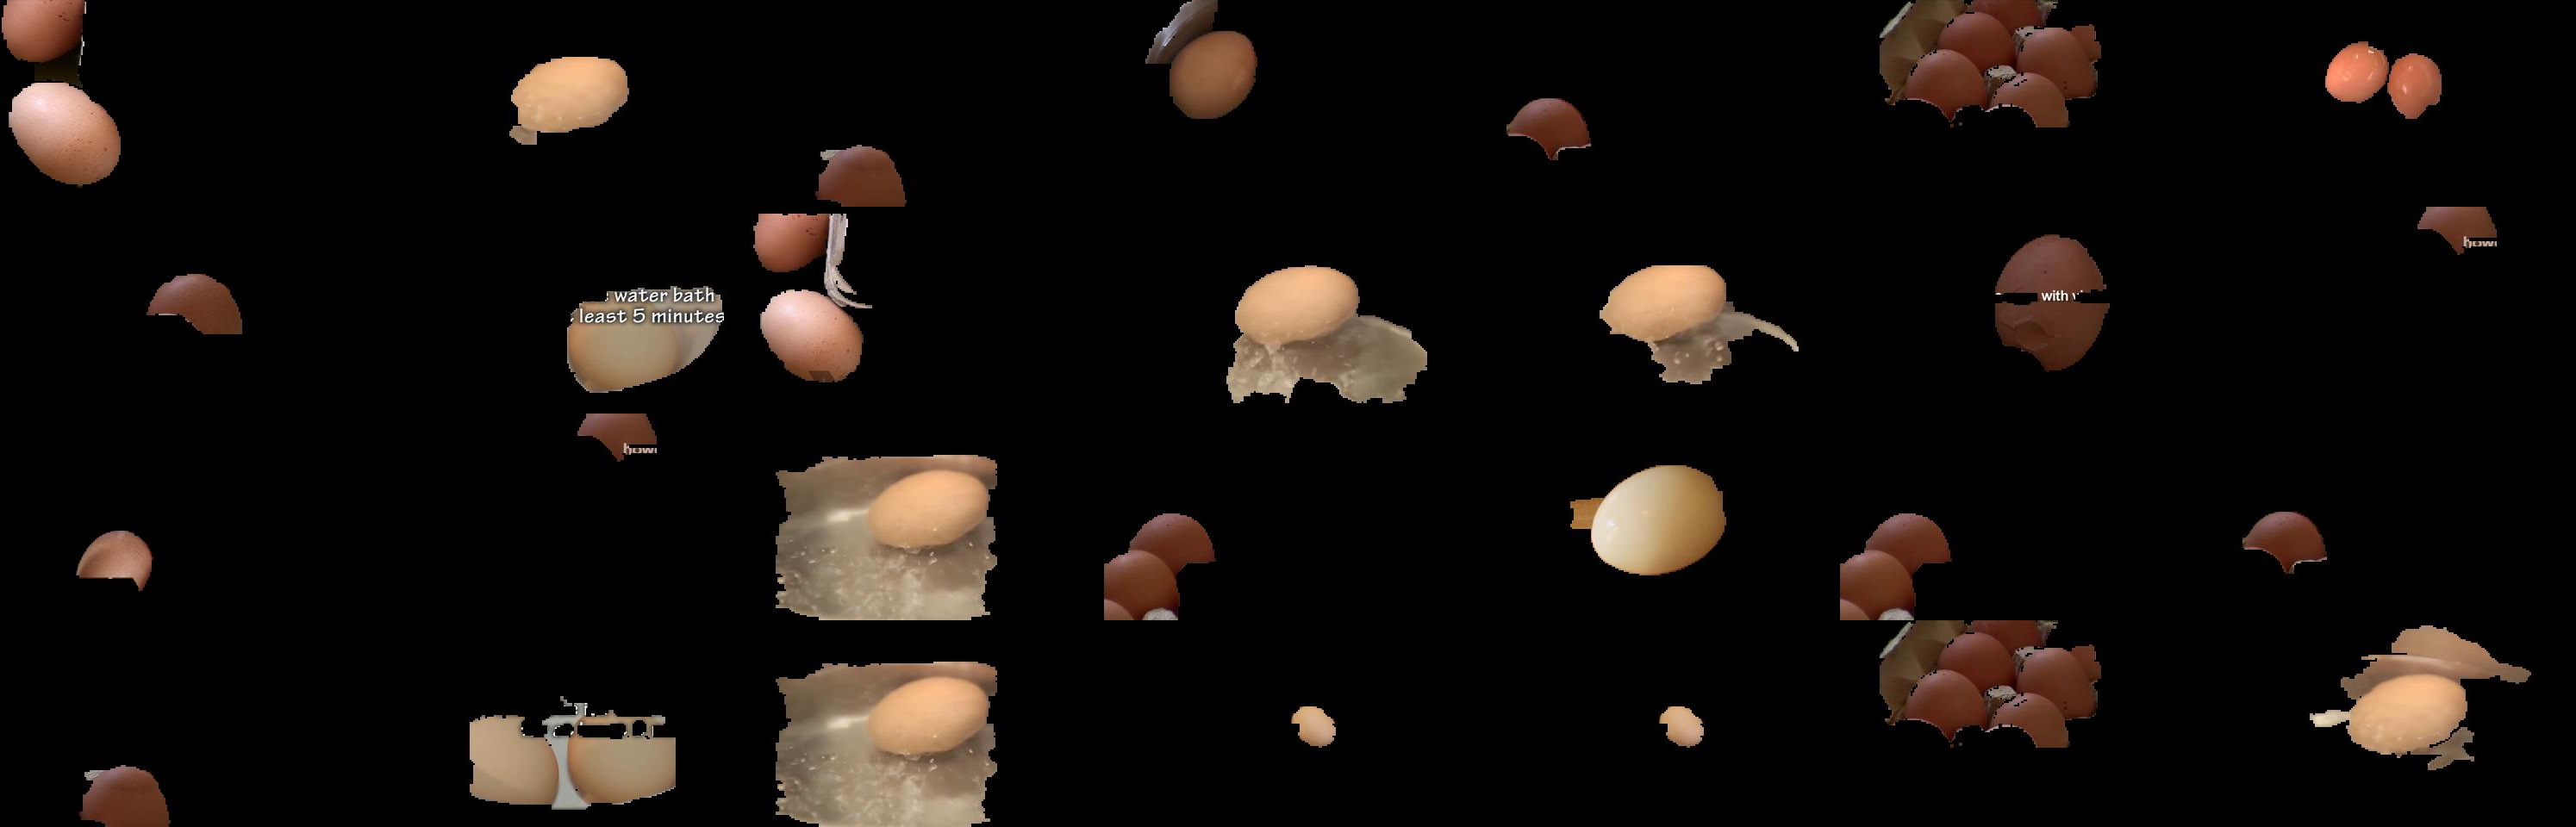
\includegraphics[width=\textwidth]{im4.png}
%\caption{Cluster 2}
\end{subfigure}
\begin{subfigure}[b]{0.23\textwidth}
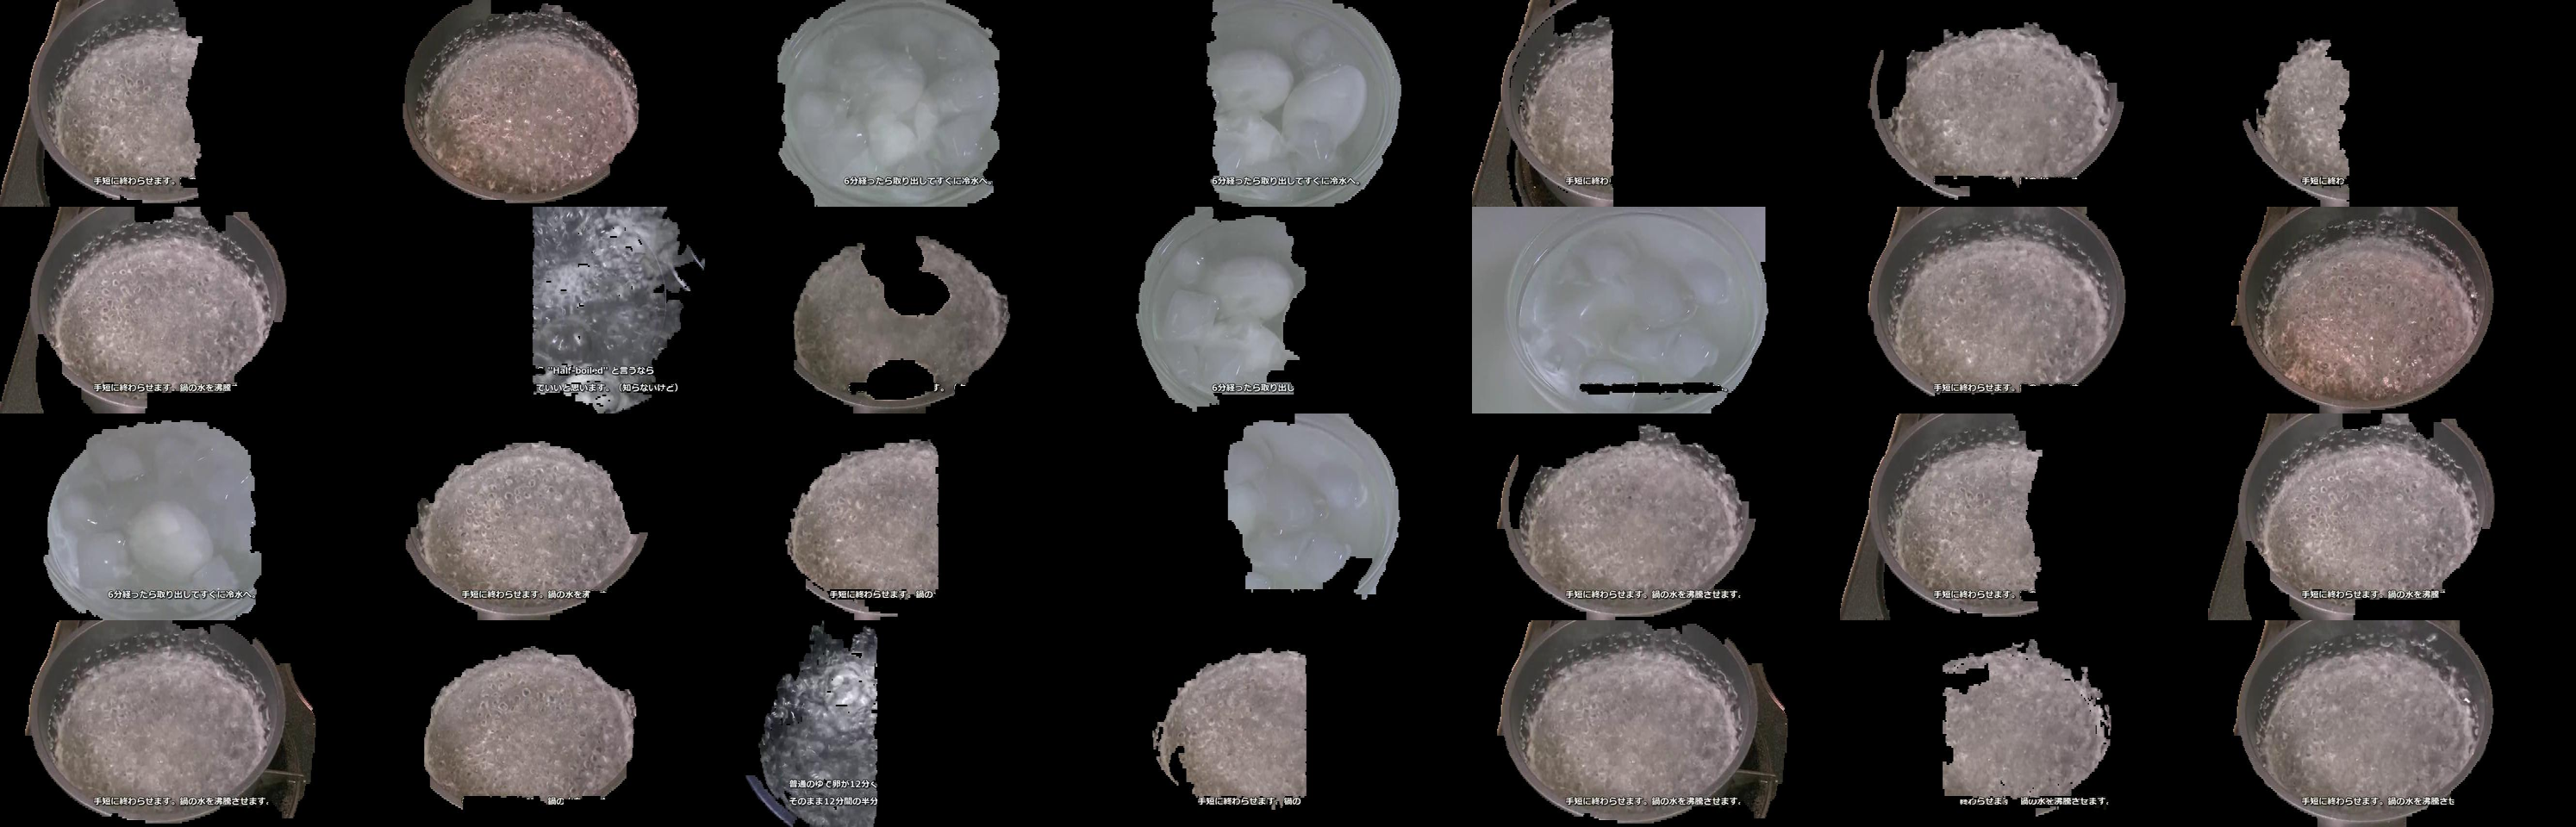
\includegraphics[width=\textwidth]{im5.png}
\end{subfigure}
~
\begin{subfigure}[b]{0.23\textwidth}
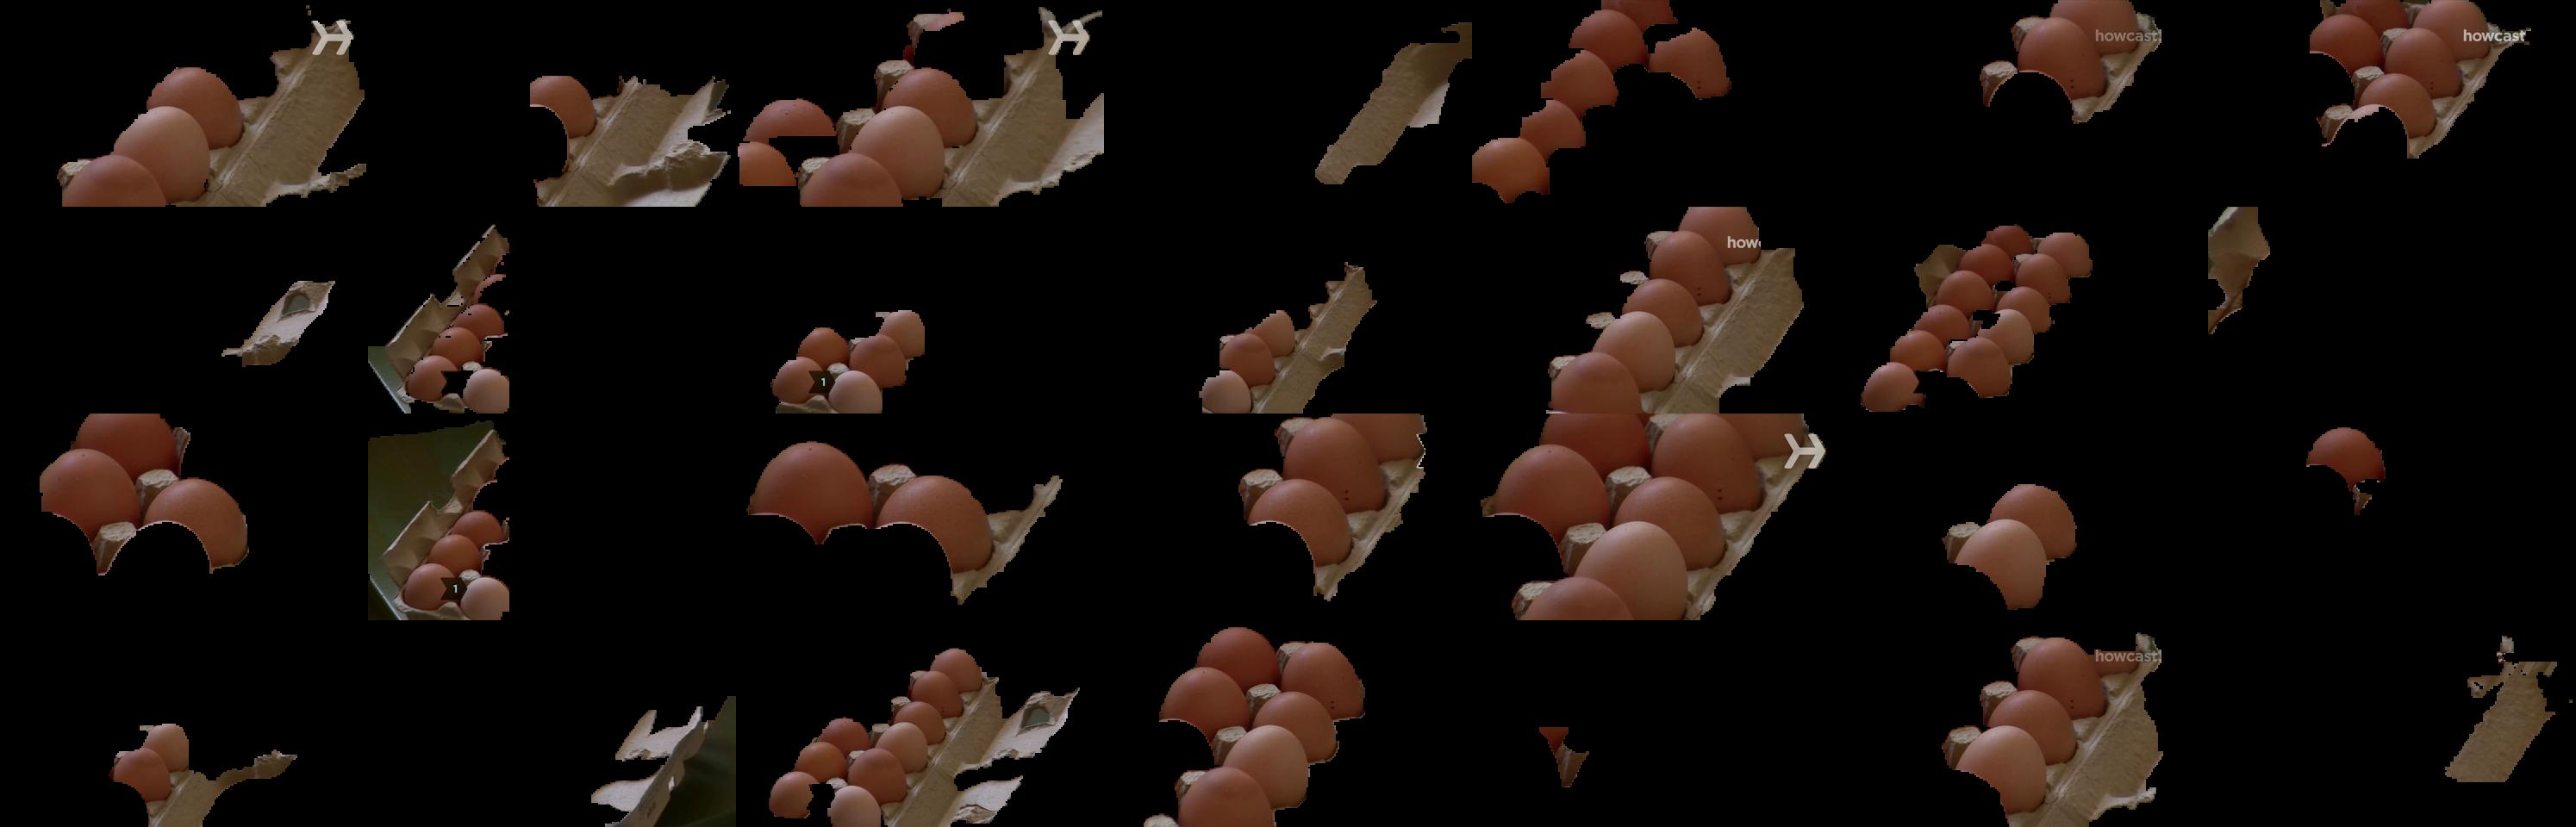
\includegraphics[width=\textwidth]{im7.png}
\end{subfigure}

\begin{subfigure}[b]{0.23\textwidth}
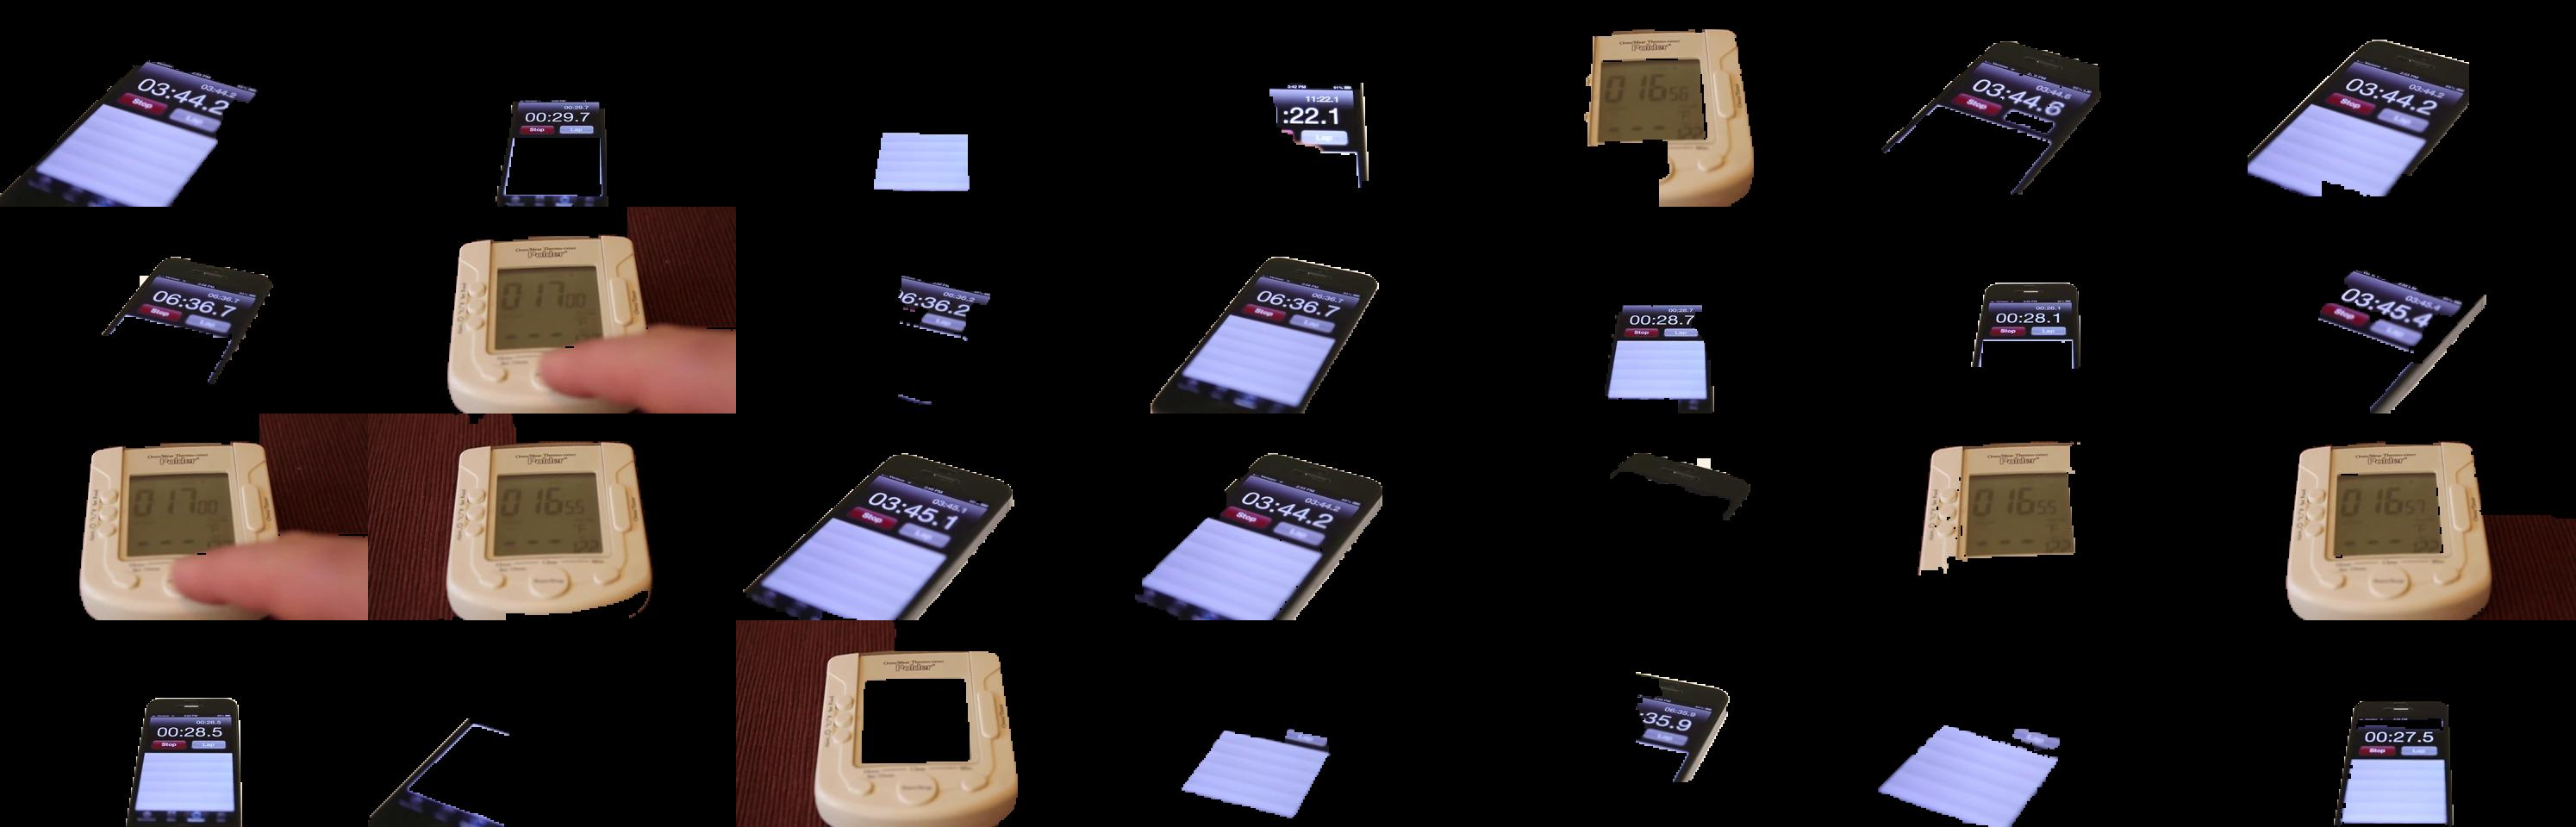
\includegraphics[width=\textwidth]{im8.png}
\end{subfigure}
~
\begin{subfigure}[b]{0.23\textwidth}
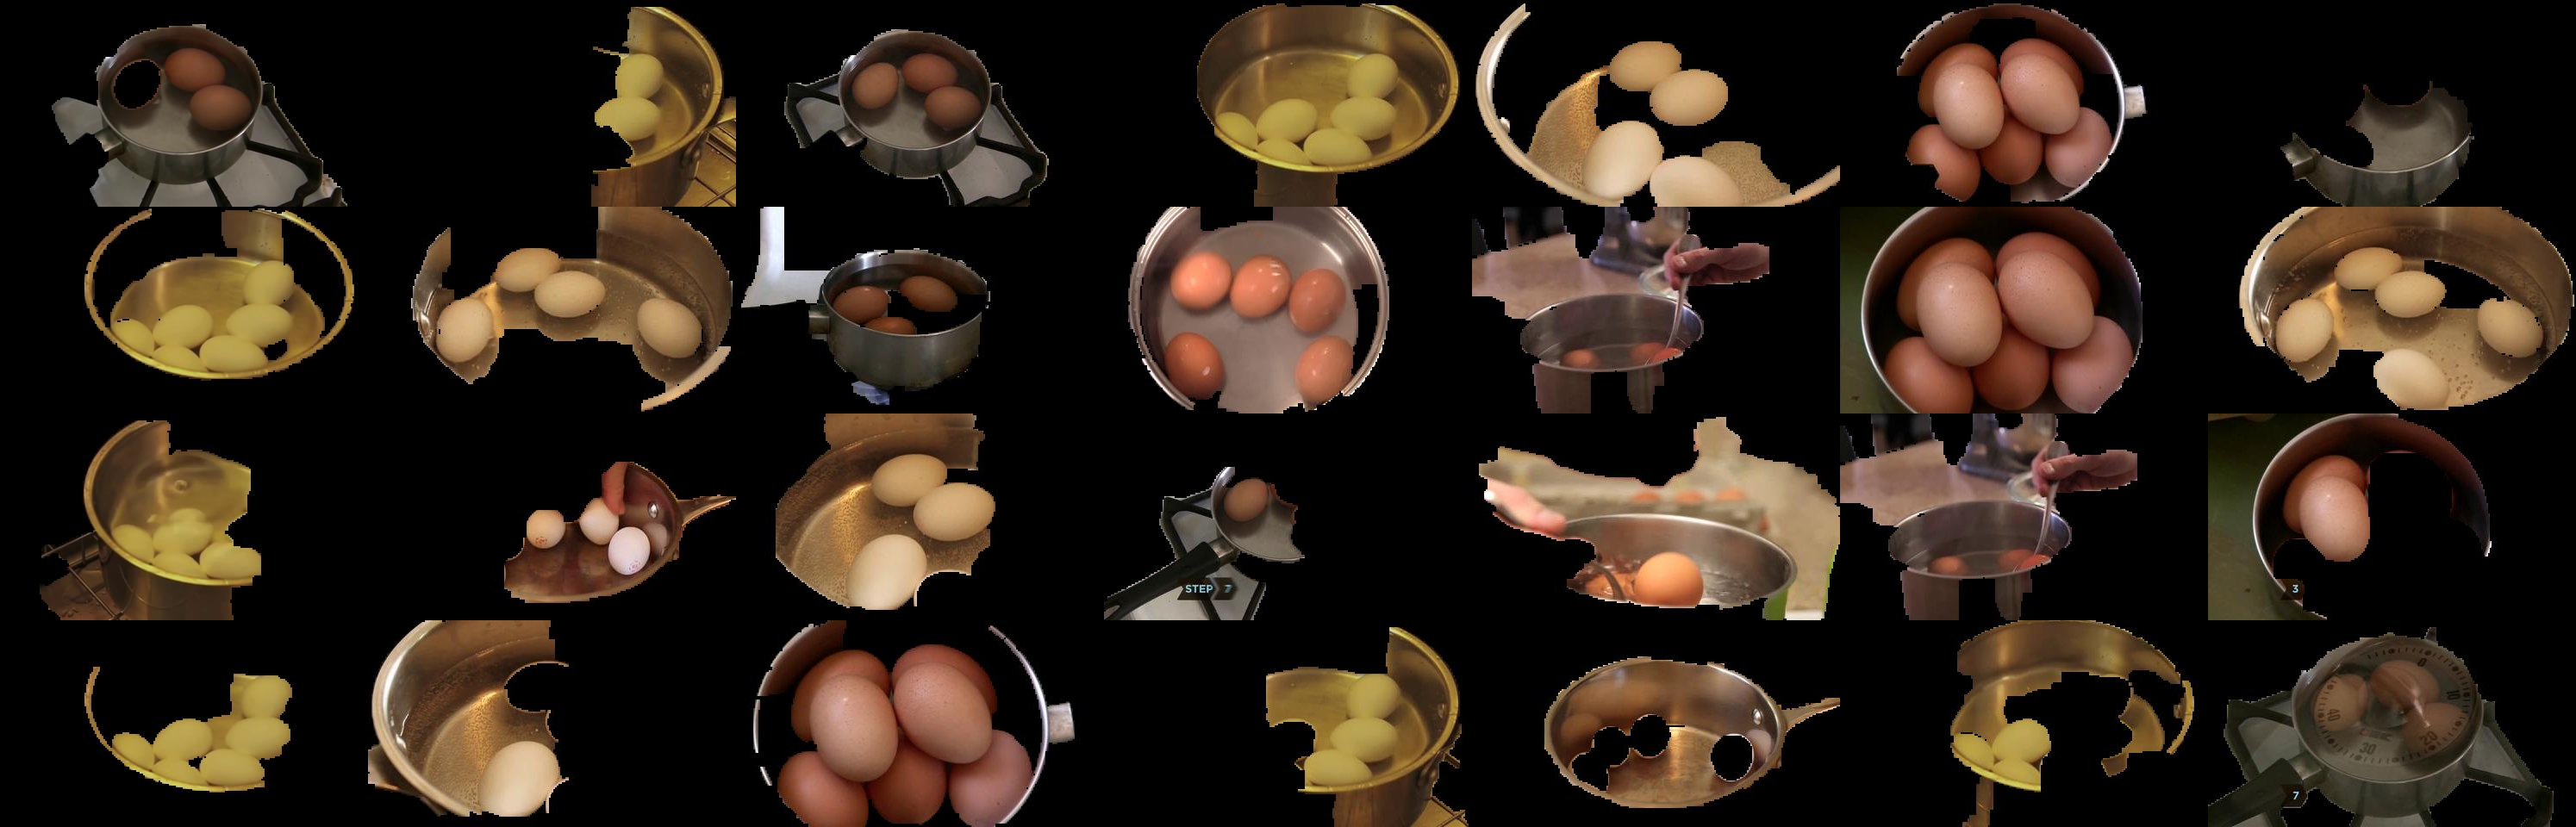
\includegraphics[width=\textwidth]{im10.png}
\end{subfigure}
\caption{Randomly selected images of randomly selected clusters learned for \emph{How to boil an egg?}}
\end{figure}
\subsection{Multi-Modal Representation via Learned Atoms}
